
%(BEGIN_QUESTION)
% Copyright 2008, Tony R. Kuphaldt, released under the Creative Commons Attribution License (v 1.0)
% This means you may do almost anything with this work of mine, so long as you give me proper credit

Graph the output of this proportional-only controller, assuming a proportional band of 25\% and a control action that is direct-acting:

$$\includegraphics[width=15.5cm]{i03274x01.eps}$$

Also, calculate the {\it bias} value for this proportional-only controller, based on the data shown in the trend.

\underbar{file i03274}
%(END_QUESTION)





%(BEGIN_ANSWER)

This is a graded question -- no answers or hints given!

%(END_ANSWER)





%(BEGIN_NOTES)

A proportional band value of 25\% is equivalent to a gain of 4.  Knowing this, we may calculate the bias value for the proportional control formula by plugging in known values of PV, SP, and Output at any given time.  Since we are only given all three values at the very start of the trend, we must use the following:

\begin{itemize}
\item{} PV = 35\%
\item{} SP = 40\%
\item{} Output = 50\%
\end{itemize}

Our formula for this direct-acting controller is as follows:

$$m = 4(\hbox{PV} - \hbox{SP}) + b$$

Solving for $b$ at those PV, SP, and Output values yields a bias of 70\%.

\vskip 10pt

A direct method of solving for the output graph is to re-calculate the output value using the proportional controller equation ($m = K_p e + b$), at every point where there is a unique PV and/or SP value.  This involves repeated calculations, which may be tedious for a complex graph.  

As an aid to doing these repeated calculations, try setting up a computer spreadsheet (e.g. Microsoft Excel) to evaluate the proportional control equation for you, and then see if you can configure the spreadsheet to produce a graph of the same PV, SP, and Output trends as well!

$$\includegraphics[width=15.5cm]{i03274x02.eps}$$


%INDEX% Control, proportional: graphing controller response

%(END_NOTES)


